\section{Taylor and Maclaurin Series Expansions}

\begin{definitionbox}[Taylor and Maclaurin Series]
If a function $f$ is infinitely differentiable in the neighborhood of a point $a$, its \textbf{Taylor series} centered at $a$ is defined as:
$$ f(x) = \sum_{k=0}^{\infty} \frac{f^{(k)}(a)}{k!} (x-a)^k $$
where $f^{(k)}(a)$ is the $k$-th derivative of $f$ evaluated at $a$.
\newline
\newline
In the special case where $\mathbf{a=0}$, the series is called a \textbf{Maclaurin series}.
\end{definitionbox}

\subsection{The Intuition Behind Taylor Series}

\begin{intuitionbox}[Building a Function from Local Information]
Imagine you are standing at a single point on the graph of a complex function, say at $x=a$. You know nothing about the function's global shape, but you can gather information about your immediate vicinity. A Taylor series is a way to construct a polynomial that perfectly mimics the function at that point, using only this local information.

\textbf{Step 0: The Position (Zeroth-Order Approximation)}
\newline
The most basic information is your position. We can approximate the function by a constant value, $f(a)$. This is a flat line. It's correct at $x=a$, but wrong everywhere else.
\newline
Approximation: $P_0(x) = f(a)$.

\textbf{Step 1: The Direction (First-Order Approximation)}
\newline
Next, we gather the slope, $f'(a)$. We can now create a line that not only passes through the correct point but also moves in the correct direction. This is the tangent line, the best possible \textit{linear} approximation.
\newline
Approximation: $P_1(x) = f(a) + f'(a)(x-a)$.

\textbf{Step 2: The Curvature (Second-Order Approximation)}
\newline
A line is straight, but the function might be curving. We measure this curvature with the second derivative, $f''(a)$. By adding a quadratic term, $\frac{f''(a)}{2}(x-a)^2$, we create a parabola that not only matches the position and slope, but also the "bend" of the function. This parabola "hugs" the function much more closely than the line did. The factor of $1/2$ (or $1/2!$) is a normalization constant that ensures the second derivative of our polynomial at $x=a$ is exactly $f''(a)$.

\textbf{The General Idea}
\newline
Each successive derivative, $f^{(k)}(a)$, provides a finer detail about the function's local shape. By adding the term $\frac{f^{(k)}(a)}{k!}(x-a)^k$, we force our polynomial's $k$-th derivative to match the function's $k$-th derivative at the point $a$. An infinite sum of these terms allows the polynomial to perfectly replicate the function in the neighborhood of $a$.
\end{intuitionbox}


\begin{definitionbox}[Taylor and Maclaurin Series]
If a function $f$ is infinitely differentiable in the neighborhood of a point $a$, its \textbf{Taylor series} centered at $a$ is defined as:
$$ f(x) = \sum_{k=0}^{\infty} \frac{f^{(k)}(a)}{k!} (x-a)^k $$
where $f^{(k)}(a)$ is the $k$-th derivative of $f$ evaluated at $a$.
\newline
\newline
In the special case where $\mathbf{a=0}$, the series is called a \textbf{Maclaurin series}. This is the most common form, as it approximates functions around the origin.
\end{definitionbox}


\subsection{The Exponential Function ($e^x$)}

\begin{theorembox}[Maclaurin Series for $e^x$]
For any real number $x$, the exponential function can be written as:
$$ e^x = \sum_{k=0}^{\infty} \frac{x^k}{k!} = 1 + x + \frac{x^2}{2!} + \frac{x^3}{3!} + \frac{x^4}{4!} + \cdots $$
\end{theorembox}

\begin{intuitionbox}[Visualizing Exponential Growth]
The exponential function is unique because it is its own derivative. This means all its local information (value, slope, curvature) at $a=0$ is equal to \textbf{1}. The series for $e^x$ is therefore the "purest" polynomial, where each term $x^k$ is simply normalized by $k!$. The graph below shows how the Taylor polynomials rapidly converge to the true exponential curve, illustrating its powerful growth.

\tcblower

\centering
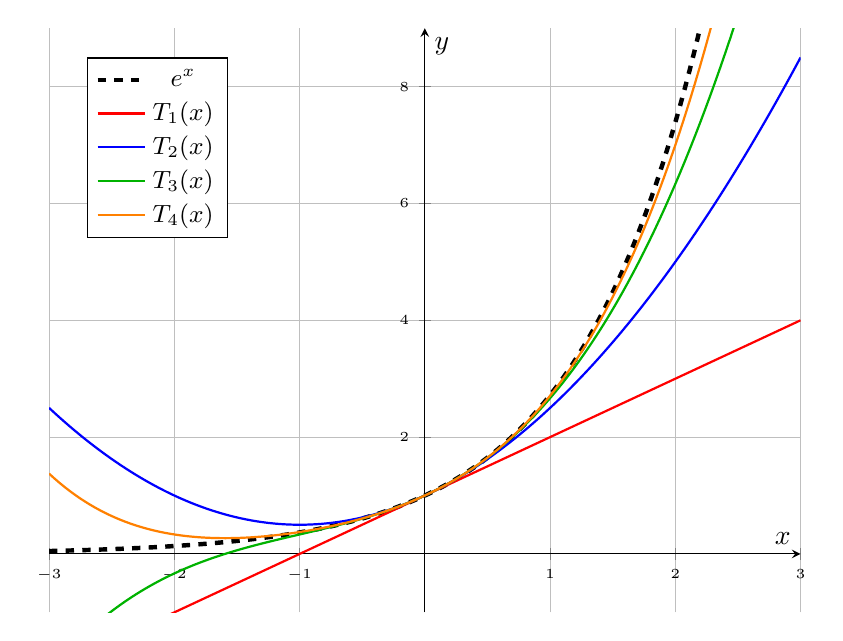
\begin{tikzpicture}
    \begin{axis}[
        xlabel={$x$},
        ylabel={$y$},
        xmin=-3, xmax=3,
        ymin=-1, ymax=9,
        axis lines=middle,
        legend style={at={(0.05,0.95)}, anchor=north west, font=\small},
        grid=major,
        samples=150,
        domain=-3:3,
        height=9cm,
        width=\linewidth-1cm,
        tick label style={font=\tiny}
    ]
    
    \addplot[black, dashed, ultra thick] {exp(x)};
    \addlegendentry{$e^x$}

    \addplot[red, thick] {1+x};
    \addlegendentry{$T_1(x)$}

    \addplot[blue, thick] {1+x+x^2/2};
    \addlegendentry{$T_2(x)$}

    \addplot[green!70!black, thick] {1+x+x^2/2+x^3/6};
    \addlegendentry{$T_3(x)$}

    \addplot[orange, thick] {1+x+x^2/2+x^3/6+x^4/24};
    \addlegendentry{$T_4(x)$}

    \end{axis}
\end{tikzpicture}
\par\small\textit{Approximation of $e^x$ by its Maclaurin polynomials.}
\end{intuitionbox}

\begin{proofbox}
Let $f(x) = e^x$. For any integer $k \ge 0$, the $k$-th derivative is $f^{(k)}(x) = e^x$. Evaluating at $a=0$, we get $f^{(k)}(0) = e^0 = 1$ for all $k$. Applying the Maclaurin formula:
$$ e^x = \sum_{k=0}^{\infty} \frac{f^{(k)}(0)}{k!} x^k = \sum_{k=0}^{\infty} \frac{1}{k!} x^k = 1 + x + \frac{x^2}{2} + \frac{x^3}{6} + \cdots $$
\end{proofbox}


\subsection{The Sine Function ($\sin(x)$)}

\begin{theorembox}[Maclaurin Series for $\sin(x)$]
For any real number $x$:
$$ \sin(x) = \sum_{k=0}^{\infty} (-1)^k \frac{x^{2k+1}}{(2k+1)!} = x - \frac{x^3}{3!} + \frac{x^5}{5!} - \frac{x^7}{7!} + \cdots $$
\end{theorembox}

\begin{intuitionbox}[Visualizing Sine's Oscillation]
The series for sine reflects its core properties. As an \textbf{odd} function ($ \sin(-x) = -\sin(x) $), its expansion contains only \textbf{odd} powers of $x$. The alternating signs capture its oscillatory nature. The graph below shows how adding terms allows the polynomial to "hug" the sine curve over more periods.

\tcblower

\centering
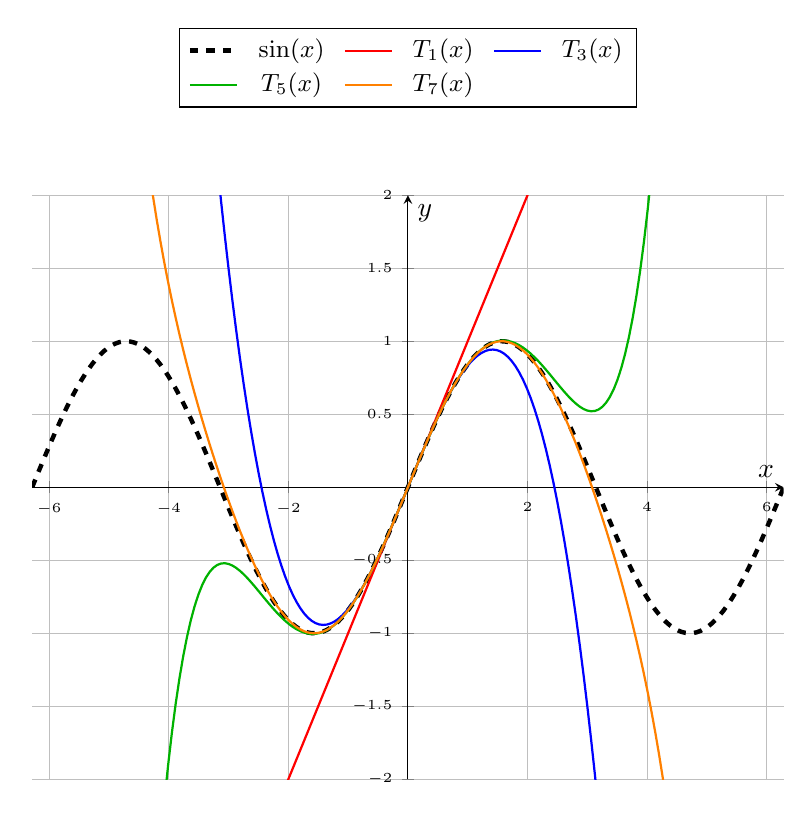
\begin{tikzpicture}
    \begin{axis}[
        xlabel={$x$},
        ylabel={$y$},
        xmin=-2*pi, xmax=2*pi,
        ymin=-2.0, ymax=2.0,
        axis lines=middle,
        legend style={at={(0.5,1.15)}, anchor=south, font=\small, column sep=5pt},
        legend columns=3,
        grid=major,
        samples=200,
        domain=-2*pi:2*pi,
        height=9cm,
        width=\linewidth-1cm,
        tick label style={font=\tiny}
    ]
    \addplot[black, dashed, ultra thick] {sin(deg(x))};
    \addlegendentry{$\sin(x)$}
    \addplot[red, thick] {x};
    \addlegendentry{$T_1(x)$}
    \addplot[blue, thick] {x - (x^3)/6};
    \addlegendentry{$T_3(x)$}
    \addplot[green!70!black, thick] {x - (x^3)/6 + (x^5)/120};
    \addlegendentry{$T_5(x)$}
    \addplot[orange, thick] {x - (x^3)/6 + (x^5)/120 - (x^7)/5040};
    \addlegendentry{$T_7(x)$}
    \end{axis}
\end{tikzpicture}
\par\small\textit{Approximation of $\sin(x)$ by its Maclaurin polynomials.}
\end{intuitionbox}

\begin{proofbox}
Let $f(x) = \sin(x)$. The derivatives at $a=0$ cycle through $(0, 1, 0, -1, \dots)$. Only odd-ordered terms ($2k+1$) are non-zero, with values of $(-1)^k$, yielding the formula.
\end{proofbox}


\subsection{The Cosine Function ($\cos(x)$)}

\begin{theorembox}[Maclaurin Series for $\cos(x)$]
For any real number $x$:
$$ \cos(x) = \sum_{k=0}^{\infty} (-1)^k \frac{x^{2k}}{(2k)!} = 1 - \frac{x^2}{2!} + \frac{x^4}{4!} - \frac{x^6}{6!} + \cdots $$
\end{theorembox}

\begin{intuitionbox}[Visualizing Cosine's Symmetry]
As an \textbf{even} function ($ \cos(-x) = \cos(x) $), the series for cosine fittingly contains only \textbf{even} powers of $x$. It starts at 1 (its maximum) and then oscillates, a behavior captured by the alternating signs.

\tcblower

\centering
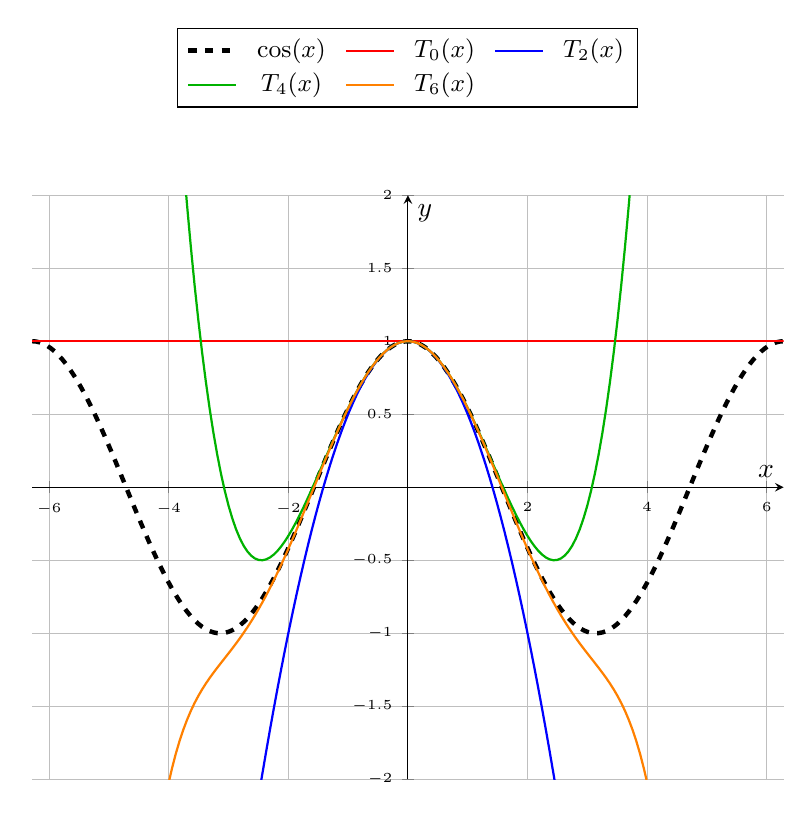
\begin{tikzpicture}
    \begin{axis}[
        xlabel={$x$},
        ylabel={$y$},
        xmin=-2*pi, xmax=2*pi,
        ymin=-2.0, ymax=2.0,
        axis lines=middle,
        legend style={at={(0.5,1.15)}, anchor=south, font=\small, column sep=5pt},
        legend columns=3,
        grid=major,
        samples=200,
        domain=-2*pi:2*pi,
        height=9cm,
        width=\linewidth-1cm,
        tick label style={font=\tiny}
    ]
    \addplot[black, dashed, ultra thick] {cos(deg(x))};
    \addlegendentry{$\cos(x)$}
    \addplot[red, thick] {1};
    \addlegendentry{$T_0(x)$}
    \addplot[blue, thick] {1 - x^2/2};
    \addlegendentry{$T_2(x)$}
    \addplot[green!70!black, thick] {1 - x^2/2 + x^4/24};
    \addlegendentry{$T_4(x)$}
    \addplot[orange, thick] {1 - x^2/2 + x^4/24 - x^6/720};
    \addlegendentry{$T_6(x)$}
    \end{axis}
\end{tikzpicture}
\par\small\textit{Approximation of $\cos(x)$ by its Maclaurin polynomials.}
\end{intuitionbox}

\begin{proofbox}
Let $g(x) = \cos(x)$. The derivatives at $a=0$ cycle through $(1, 0, -1, 0, \dots)$. Only even-ordered terms ($2k$) are non-zero, with values of $(-1)^k$, yielding the formula.
\end{proofbox}


\subsection{The Natural Logarithm ($\ln(1+x)$)}

\begin{theorembox}[Maclaurin Series for $\ln(1+x)$]
For $|x| < 1$:
$$ \ln(1+x) = \sum_{k=1}^{\infty} (-1)^{k-1} \frac{x^k}{k} = x - \frac{x^2}{2} + \frac{x^3}{3} - \frac{x^4}{4} + \cdots $$
\end{theorembox}

\begin{intuitionbox}[Visualizing Logarithmic Approximation]
This series is essential for approximating logarithms near 1. Unlike the previous functions, it only converges for $|x|<1$. The graph shows that the approximation is excellent near $x=0$ but diverges rapidly as $x$ approaches the boundary of convergence at $x=1$.

\tcblower

\centering
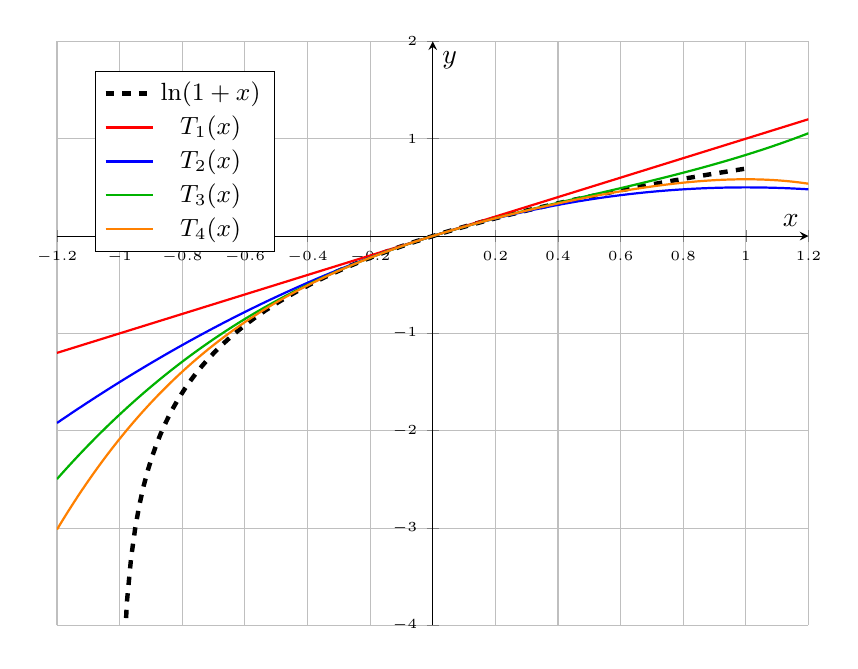
\begin{tikzpicture}
    \begin{axis}[
        xlabel={$x$},
        ylabel={$y$},
        xmin=-1.2, xmax=1.2,
        ymin=-4, ymax=2,
        axis lines=middle,
        legend style={at={(0.05,0.95)}, anchor=north west, font=\small},
        grid=major,
        samples=150,
        domain=-0.99:1, % Domain restricted for ln
        height=9cm,
        width=\linewidth-1cm,
        tick label style={font=\tiny}
    ]
    \addplot[black, dashed, ultra thick] {ln(1+x)};
    \addlegendentry{$\ln(1+x)$}
    
    \addplot[red, thick, domain=-1.2:1.2] {x};
    \addlegendentry{$T_1(x)$}

    \addplot[blue, thick, domain=-1.2:1.2] {x - x^2/2};
    \addlegendentry{$T_2(x)$}

    \addplot[green!70!black, thick, domain=-1.2:1.2] {x - x^2/2 + x^3/3};
    \addlegendentry{$T_3(x)$}
    
    \addplot[orange, thick, domain=-1.2:1.2] {x - x^2/2 + x^3/3 - x^4/4};
    \addlegendentry{$T_4(x)$}

    \end{axis}
\end{tikzpicture}
\par\small\textit{Approximation of $\ln(1+x)$ by its Maclaurin polynomials.}
\end{intuitionbox}

\begin{proofbox}
Let $f(x) = \ln(1+x)$. For $k \ge 1$, the $k$-th derivative at $a=0$ is $f^{(k)}(0) = (-1)^{k-1} (k-1)!$. Substituting this into the Maclaurin formula, the $(k-1)!$ in the numerator partially cancels the $k!$ in the denominator, leaving a $k$ on the bottom.
\end{proofbox}